\section{Árboles de Sintáxis Abstracta en Golang}
\textit{Golang} provee una serie de paquetes que permiten trabajar con el código fuente escrito en ese 
lenguaje de programación, facilitando la creación de \textbf{árboles de sintáxis abstracta}
(o \textbf{ASTs} por sus siglas en inglés), para el análisis o manipulación de los mismos.
Al ser provisto oficialmente por los creadores dentro del conjunto estándar de herramientas, 
no es necesario definir la gramática para alguna otra herramienta como ANTLR.
Además, esto nos asegura que se soportan todas las estructuras que componen el lenguaje 
y se encuentran definidas en la especificación del mismo [AGREGAR REFERENCIA].

\begin{figure}[H]
  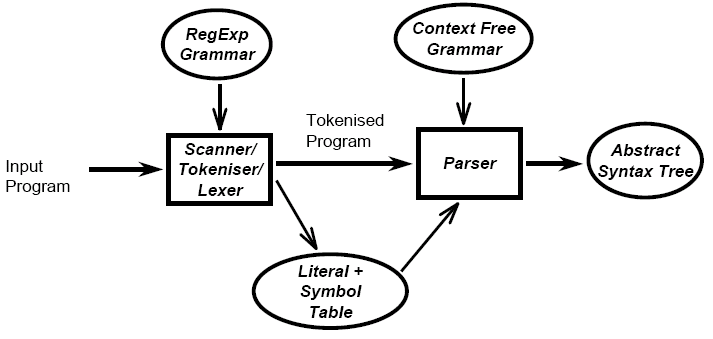
\includegraphics[width=12cm]{implementation/parsingpipeline}
  \centering
  \caption{Creación de un AST desde código fuente}
\end{figure}

En la figura X se establece la correlación entre las etapas del proceso de creación de un AST 
a partir de código fuente y los paquetes provistos en el lenguaje de programación.
La función de cada uno de estos, y su participación en el proceso, se indica a continuación:
\begin{itemize}
  \item \textbf{go/token} Contiene el conjunto de \textit{tokens} del léxico que conforman el 
  lenguaje de programación Go, junto con las operaciones que pueden aplicarse a los mismos.
  \item \textbf{go/scanner} El paquete \textit{scanner} ofrece las estructuras, interfaces y 
  funciones necesarias para tokenizar una cadena de texto que represente un fragmento o 
  archivo de código fuente de Go.
  \item \textbf{go/ast} Es el paquete donde se especifican las estructuras y tipos de datos para 
  representar los elementos del árbol de sintaxis abstracta, al igual que las operaciones aplicables 
  sobre los mismos.
  Las principales estructuras y funciones de este paquete son:
  \begin{itemize}
    \item \textbf{Visitor} Es la interfaz que define el contrato que tiene que cumplir una estructura 
    para considerarse Visitor, y especifica una función \textit{Visit}, la cual se utiliza para 
    recorrer el AST, y recibe un nodo del mismo como parámetro.
    El argumento de salida de esta función es otro elemento que cumple la interfaz \textit{Visitor}.
    \item \textbf{Node} Es una interfaz que implementan todos los elementos que componen un AST, y 
    define el contrato para identificar el inicio y fin del nodo a nivel de tokens.
    \item \textbf{Walk(v Visitor, node Node)} Esta función recorre el AST, nodo por nodo, siguiendo 
    el enfoque de \textit{depth-first}.
    El proceso comienza cuando se llama a \textit{v.Visit(node)}, y si este no es nulo, procede 
    recursivamente llamando a esa función con cada uno de los hijos no nulos.
    En caso de alcanzar un nodo final, la visita a éste retorna nulo y así puede volver sobre el árbol 
    y continuar con los nodos de otro nivel.
  \end{itemize}
  \item \textbf{go/parser} El paquete contiene las funciones y configuraciones necesarias para el \textit{parsing} 
  de código fuente sea a través de directorios, archivos o directamente expresiones. 
  Cabe destacar que, el \textit{parsing}, aplica y reconoce solamente la sintaxis de Go.
  El resultado del parseo es un árbol de sintáxis abstracta (AST), el cual puede luego ser procesado 
  para evaluar, extraer información e incluso modificarlo.
  Los principales elementos de este paquete son:
  \begin{itemize}
    \item \textbf{ParseFile(fset *token.FileSet, filename string, src interface{}, mode Mode) (f *ast.File, err error)} 
    Es la función realiza el parseo de un sólo archivo de Go y retorna el nodo correspondiente a \textbf{ast.File}.
    El elemento devuelto representa solamente el archivo en cuestión, sin tener en cuenta el resto de 
    archivos que compone el paquete/proyecto, por lo que para obtener el árbol completo del proyecto, 
    es necesario combinar los resultados de cada una de sus llamadas.
    El primer argumento de entrada, de tipo \textit{token.FileSet}, representa un conjunto de archivos 
    y métodos para acceder de forma sincronizada a los mismos, evitando inconvenientes por concurrencia.
    Los argumentos de entrada \textit{filename} y \textit{src} indican cuál será el archivo a procesar.
    El primero, lo hace a través del nombre del archivo; mientras que el segundo se utiliza para brindar 
    directamente el contenido del mismo.
    Por último, \textit{mode} configura cómo debe correr el parser para esa ejecución.
    \item \textbf{Mode} Es un indicador de cuánto código debe importarse, junto con otras opciones para el parser.
    Permite establecer diferentes niveles de importación, como por ejemplo sólo la definición del paquete, 
    las importaciones, la inclusión de comentarios y el tratamiento de errores.
  \end{itemize}
\end{itemize}
